\documentclass[12pt]{article}

\usepackage{sbc-template}
\usepackage{graphicx,url}
\usepackage{babel}
\usepackage[T1]{fontenc}
\usepackage[utf8]{inputenc}
\usepackage{multicol}
\usepackage{multirow}
\usepackage{amsmath,amssymb,amsfonts}
\usepackage{textcomp}
\usepackage{url}
\usepackage{enumerate}
\usepackage{verbatim}
\usepackage[table,xcdraw]{xcolor}
\usepackage[shortlabels]{enumitem}
\usepackage{fancyhdr}
\usepackage{sbgames}
\usepackage{booktabs}
\usepackage{tikz}
\usetikzlibrary{positioning,arrows.meta,shapes.geometric}

\tolerance=1
\emergencystretch=\maxdimen
\hyphenpenalty=10000
\hbadness=10000

\sloppy


\trilha{Informe a Trilha} %Preencha com: Artes \& Design | Computação | Cultura | Saúde | Indústria | Educação | Tutoriais | MAGICA | WGP-Jogos
\local{Cidade/UF} % Exemplo: Manaus/AM
\ano{20XX} % Exemplo: 2024
\edicao{Edição (Romano)} %Exemplo: XXIII

\title{Avaliação de Sistemas Interativos Baseados em LLM: Um Protocolo Reprodutível para Coerência Narrativa e Consistência de Estado \\
\medskip
\small{
    \textit{Title: Evaluating Interactive LLM-Based Systems: A Reproducible Protocol for Narrative Coherence and State Consistency}
}
}

\author{[OMITIDO PARA REVISÃO ANÔNIMA]}

\address{[OMITIDO PARA REVISÃO ANÔNIMA]
  \email{[OMITIDO PARA REVISÃO ANÔNIMA]}
}

\begin{document}

\maketitle

\thispagestyle{plain}

\begin{abstract}
Evaluating interactive Large Language Model (LLM)-based systems --- such as Game Masters in role-playing games (RPGs) --- remains a challenging problem due to the multi-turn, stateful, and subjective nature of these interactions. This paper presents a reproducible evaluation protocol for interactive LLM-based systems, based on LLM-as-a-judge, operating over structured gameplay logs. The proposed method defines a metric-driven pipeline that captures key dimensions of system performance, including narrative quality, action-to-narration coherence, and state consistency. Unlike prior approaches focused on static or controlled benchmarks, the protocol evaluates full gameplay sessions, enabling analysis of long-term behavior and state evolution. The system supports local LLM deployment, ensuring reproducibility and independence from external services. We observe that the protocol effectively differentiates system performance across four open-weight models (Qwen2.5 family at 0.5B, 1.5B and 7B; Gemma 4 effective 2B) over 10 sessions with 3 human players (30--60 rounds each), and identifies five recurring failure modes, including internal-variable leakage, history-contamination hallucinations, persona breaks with meta-apologies, and exposure of system prompt structure --- all more frequent in models below 7B parameters. The proposed protocol provides a practical and extensible framework for evaluating interactive, stateful LLM-based systems.
\end{abstract}

\keywords{Large Language Models, Game AI, Evaluation Methods, Interactive Systems, Narrative Generation, LLM-as-a-Judge.}

\begin{resumo}
A avaliação de sistemas interativos baseados em Modelos de Linguagem de Grande Escala (LLMs) --- como Mestres de Jogo em RPGs --- é um problema desafiador devido à natureza multi-turno, com estado e subjetiva dessas interações. Este trabalho apresenta um protocolo reprodutível de avaliação para sistemas interativos baseados em LLM, fundamentado em LLM-as-a-judge e operando sobre logs estruturados de \textit{gameplay}. O método propõe um pipeline orientado a métricas que capta dimensões-chave de desempenho --- qualidade narrativa, coerência ação--narração e consistência de estado. Diferente de abordagens centradas em \textit{benchmarks} estáticos ou controlados, o protocolo avalia sessões completas de jogo, viabilizando análise de comportamento de longo prazo e evolução de estado. O sistema suporta execução local, garantindo reprodutibilidade e independência de serviços externos. Resultados experimentais com quatro modelos de pesos abertos (Qwen2.5 em 0.5B, 1.5B e 7B; Gemma~4 effective~2B) e 3 jogadores humanos (10 sessões, 30--60 rodadas cada) demonstram que o protocolo diferencia consistentemente o desempenho dos sistemas e identifica cinco modos recorrentes de falha, incluindo vazamento de variáveis internas, alucinações por contaminação de histórico, quebra de persona com meta-desculpas e exposição da estrutura do prompt de sistema --- todos mais frequentes em modelos abaixo de 7B parâmetros. O protocolo proposto fornece um arcabouço prático e extensível para avaliação de sistemas interativos baseados em LLM com estado.
\end{resumo}

\palavraschave{Modelos de Linguagem, IA em Jogos, Métodos de Avaliação, Sistemas Interativos, Geração Narrativa, LLM-as-a-Judge.}

% ─────────────────────────────────────────────────────────────────────────────
\section{Introdução}

Jogos de RPG de mesa (\textit{tabletop RPG}) dependem de um Mestre de Jogo (MJ) humano para conduzir a narrativa, arbitrar regras e manter a consistência do mundo. Com o avanço dos Grandes Modelos de Linguagem (LLMs), tornou-se possível automatizar parcialmente essas funções, criando MJs artificiais capazes de gerar narrativas interativas.

No entanto, a \textbf{avaliação} desses sistemas permanece um desafio aberto. A qualidade narrativa, a coerência entre ações e descrições e a consistência de estado ao longo de múltiplas interações são aspectos difíceis de mensurar objetivamente. Métodos tradicionais baseados em avaliação humana apresentam limitações de escalabilidade, custo e reprodutibilidade.

Visando automatizar essa tarefa, trabalhos recentes propõem o uso de LLM como avaliadores (\textit{LLM-as-a-judge}), possibilitando a análise automática de textos gerados. Em particular, o RPGBench \cite{yu:2025} introduz métricas específicas para sistemas de RPG baseados em LLM. Contudo, essas abordagens são geralmente aplicadas a cenários controlados e não a sessões interativas completas com múltiplos turnos.

Este trabalho propõe um pipeline de avaliação automática aplicado a sessões reais de RPG, utilizando logs estruturados e métricas adaptadas do RPGBench. A principal contribuição deste trabalho é um \textbf{protocolo de avaliação reprodutível para Mestres de Jogo baseados em LLM em RPGs interativos}, configurando uma \textit{extensão} da avaliação no estilo RPGBench \cite{yu:2025} para sessões interativas completas com múltiplos turnos a partir de logs estruturados. O protocolo é materializado no módulo \texttt{rpg\_judge.py} e executado integralmente em modelos locais ---eliminando dependência de serviços em nuvem--- cobrindo combate, diálogo e exploração de mundo aberto.

% ─────────────────────────────────────────────────────────────────────────────
\section{Trabalhos Relacionados}

\textbf{LLMs em Jogos.}
Gallotta et al. \cite{gallotta:2024} apresentam um \textit{survey} abrangente do uso de LLMs em jogos, identificando papéis em geração de conteúdo, controle de NPCs e narrativa interativa. Aplicações específicas a RPGs aparecem em trabalhos recentes da comunidade brasileira: \cite{sbgames:llm:2025} explora LLMs em jogos narrativos, e \cite{sbgames:tabletop:2025} aplica RAG para geração de diálogos em \textit{tabletop RPG}. Antes da popularização dos LLMs, comportamento de NPCs e coordenação multi-agente em jogos eram tipicamente modelados via Behavior Trees e regras simbólicas \cite{agis:2020}, com vantagens de previsibilidade e custo computacional, porém limitações de generalização para diálogos abertos.

\textbf{LLMs como Mestres de RPG.}
Acharya et al. \cite{acharya:2023} investigam suporte computacional baseado em LLMs para Game Masters de TTRPG, focando em assistência ao MJ humano. O presente trabalho difere ao investigar substituição autônoma do MJ, com sessão integralmente conduzida pelo LLM e avaliação automática posterior. Yu et al. \cite{yu:2025} propõem o RPGBench, \textit{benchmark} para avaliar LLMs como motores de RPG com métricas de qualidade narrativa, consistência de estado e coerência de ação. A metodologia LLM-as-a-judge é adotada neste trabalho com adaptações para o contexto brasileiro e suporte a modelos locais.

\textbf{LLM-as-a-Judge.}
Zheng et al. \cite{zheng:2023} validam o uso de LLMs como avaliadores automáticos de qualidade textual no contexto do MT-Bench, demonstrando correlação superior a 80\% com julgamento humano para tarefas abertas. Essa evidência sustenta a escolha metodológica de avaliar sessões de jogo sem participantes humanos. Uma limitação importante é o possível viés quando o mesmo modelo base é usado para geração e avaliação---ponto discutido na Seção~6. Reviriego et al. \cite{reviriego:2024} mostram que métricas de diversidade lexical (TTR, MTLD) são complementares à avaliação semântica e podem detectar degradação de qualidade não capturada por LLM-as-a-judge isolado, motivando a inclusão dessas métricas em trabalho futuro.

\textbf{Geração Procedural e Persistência.}
Shaker, Togelius e Nelson \cite{shaker:2016} oferecem o referencial canônico para o Cenário C, onde biomas, inimigos e nomes de localidades são gerados proceduralmente a partir de coordenadas espaciais $(x,y,z)$. A persistência via SQLite garante que modificações ambientais sobrevivam entre sessões, mantendo consistência narrativa estrutural independente de memória interna do modelo.

% ─────────────────────────────────────────────────────────────────────────────
\section{Arquitetura do Sistema}

\subsection{Visão Geral}

O sistema é composto por três camadas funcionais: (1) \textbf{Interface} --- questionário narrativo inicial com avaliação LLM e menu de modos; (2) \textbf{Jogo} --- motor de combate, mundo aberto e narrativa de NPCs; (3) \textbf{Persistência} --- log unificado em CSV, SQLite por coordenada e JSON de estado.

Três backends de LLM são suportados via \texttt{llm\_backend.py}: Ollama (local), Groq API (cloud gratuito) e LM Studio 0.4.11 (servidor local com API nativa \texttt{/api/v1/chat}). O backend e o modelo são lidos do arquivo \texttt{llm\_config.py} em tempo de execução a cada chamada, sem cache, permitindo troca de modelo sem reinicialização.

\subsection{Pipeline de Combate}

O Cenário A implementa um pipeline de 16 etapas por turno, incluindo: exibição de HUD com arte ASCII por subtipo de inimigo, avaliação LLM de criatividade (0--1) e eficiência (0--2), detecção de ação defensiva pura ou mista, cálculo de dano, narração em \textit{streaming}, atualização de \textit{status effects} (sangramento, veneno, paralisia), progressão de maestria de arma e registro completo no \texttt{session\_log}.

A detecção de ação defensiva diferencia ações puras (``esquiva'', ``bloqueio'') de ações mistas que combinam defesa e ataque (``preparo minha esquiva e contra-ataco''). Ações mistas são tratadas como ataque normal com componente defensivo, evitando que o jogador burle o sistema de avaliação.

\subsection{Cenário B --- Diálogo e Memória de Longo Prazo}

O Cenário B foi originalmente concebido para investigar memória de longo prazo e qualidade narrativa em diálogos investigativos com NPCs. Durante o desenvolvimento, suas funcionalidades centrais foram distribuídas organicamente entre os Cenários A e C, sem prejuízo da cobertura experimental: o diálogo livre com NPCs ocorre tanto após cada quinta batalha de bioma no Cenário A (com menu estruturado de ações: conversar, descansar, treinar, troca de item, ajuda contextual e revelação de segredo condicionada a amizade $\geq 60$) quanto continuamente no acampamento do Cenário C (comando \texttt{falar~<nome>}). Em ambos os contextos o motor é o mesmo (\texttt{NPC.falar()}), com prompt instruído a responder em primeira pessoa e em 2--4 linhas.

A memória de longo prazo é implementada em três camadas: histórico de diálogo por NPC (SQLite, \texttt{memoria\_npc.py}), estado da jornada em JSON (\texttt{jornada.py}) e fatos por coordenada (SQLite do mundo aberto). Quando o jogador retoma uma sessão, o sistema injeta o histórico anterior no prompt via \texttt{memoria\_npc.contexto\_para\_llm()}, criando o efeito de continuidade narrativa originalmente proposto para o Cenário B. As métricas GS3 (coerência ação$\to$narração) e GS6 (consistência de estado entre turnos) do \texttt{rpg\_judge.py} cobrem precisamente as dimensões que o Cenário B pretendia exercitar, sem demandar um quarto cenário separado.

\subsection{Cenário C --- Mundo Aberto}

O Cenário C implementa exploração livre em malha de coordenadas $(x,y,z)$. O bioma é determinado pela distância euclidiana à origem: floresta ($d<2$), planície ($d<5$), deserto/pântano ($d<9$), ruínas ($d>9$), caverna ($z<-2$) e montanha ($z>3$). A Tabela~\ref{tab:modificacoes} lista os tipos de modificação ambiental detectados.

\begin{table}[ht]
\centering
\caption{Modificações ambientais persistentes por coordenada no Cenário C}
\label{tab:modificacoes}
\begin{tabular}{ll}
\toprule
\textbf{Tipo} & \textbf{Palavras-chave detectadas} \\
\midrule
Fogo       & bola de fogo, incêndio, chamas \\
Corte      & corto a árvore, machado, derruba \\
Magia      & conjuro, lanço, raio arcano \\
Escavação  & cavo, escavar, picareta \\
Construção & construo, ergo, barricada \\
Gelo       & congelo, nevar, freeze \\
Explosão   & explodo, blast \\
Água       & inundo, flood \\
\bottomrule
\end{tabular}
\end{table}

Cada local visitado é persistido em SQLite com nome gerado proceduralmente, descrição LLM e histórico de modificações. Ao revisitar um local, o sistema exibe as modificações anteriores no contexto enviado à LLM, mantendo consistência narrativa sem depender de memória interna do modelo.

O \texttt{mundo\_log.csv} registra todos os eventos com campo \texttt{session\_id}, permitindo que o \texttt{rpg\_judge} avalie apenas os eventos da sessão correspondente mesmo quando múltiplas sessões compartilham o mesmo arquivo.

% ─────────────────────────────────────────────────────────────────────────────
\section{Framework de Avaliação Automática}

\subsection{Metodologia}

A avaliação segue a metodologia Design Science Research (DSR) \cite{hevner:2004,peffers:2007,pimentel:2020} em cinco fases adaptadas: identificação do problema, objetivos, design, demonstração e avaliação. Hevner et al. \cite{hevner:2004} fornecem o framework conceitual de DSR; Peffers et al. \cite{peffers:2007} formalizam o processo em etapas reutilizáveis; Pimentel, Filippo e Santos \cite{pimentel:2020} sintetizam a abordagem em português, alinhando-a ao contexto brasileiro de pesquisa. A fase de avaliação emprega sessões instrumentadas com logging automático, analisadas pelo módulo \texttt{rpg\_judge.py} via LLM-as-a-judge, conforme pipeline ilustrado na Figura~\ref{fig:pipeline}.

A avaliação experimental foi conduzida com \textbf{3 jogadores distintos}, cada um realizando ao menos 2 sessões completas (30--60 rodadas por sessão), totalizando 10 sessões avaliadas automaticamente pelo \texttt{rpg\_judge.py}. A inclusão de múltiplos jogadores introduz variância de estilo de jogo (ações livres, escolhas narrativas) e fortalece a validade externa frente a abordagens com avaliador único como em RPGBench \cite{yu:2025}. O número de sessões está em ordem de grandeza compatível com o mínimo sugerido por Yu et al.; uma bateria maior é direção de trabalho futuro.

\begin{figure}[ht]
\centering
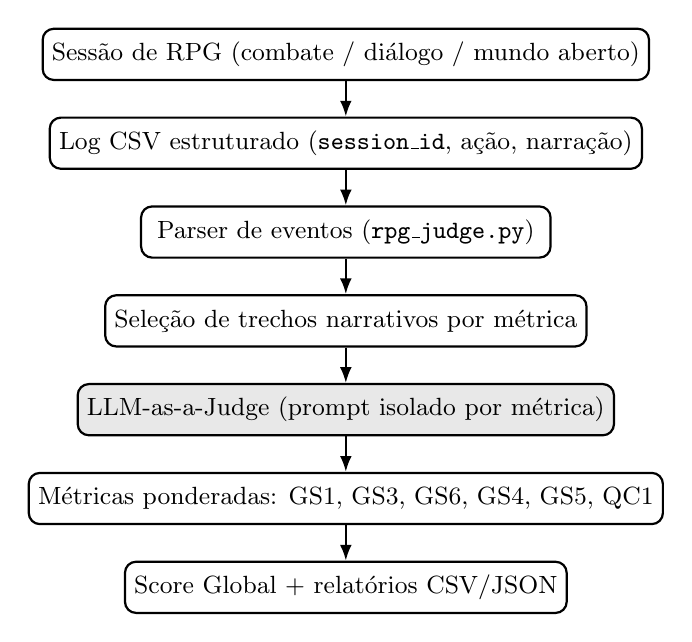
\begin{tikzpicture}[
  node distance=0.45cm,
  every node/.style={
    rectangle, rounded corners, draw=black, thick,
    minimum width=5.2cm, minimum height=0.65cm,
    align=center, font=\small
  },
  judge/.style={fill=gray!18},
  arr/.style={-{Latex[length=2mm]}, thick}
]
\node (a) {Sessão de RPG (combate / diálogo / mundo aberto)};
\node (b) [below=of a] {Log CSV estruturado (\texttt{session\_id}, ação, narração)};
\node (c) [below=of b] {Parser de eventos (\texttt{rpg\_judge.py})};
\node (d) [below=of c] {Seleção de trechos narrativos por métrica};
\node (e) [below=of d, judge] {LLM-as-a-Judge (prompt isolado por métrica)};
\node (f) [below=of e] {Métricas ponderadas: GS1, GS3, GS6, GS4, GS5, QC1};
\node (g) [below=of f] {Score Global + relatórios CSV/JSON};
\foreach \x/\y in {a/b, b/c, c/d, d/e, e/f, f/g} \draw[arr] (\x) -- (\y);
\end{tikzpicture}
\caption{Pipeline de avaliação automática baseado em LLM-as-a-judge. Logs estruturados de sessões são processados e avaliados por um modelo de linguagem segundo métricas narrativas e de consistência de estado, produzindo um relatório reprodutível independente de avaliação humana.}
\label{fig:pipeline}
\end{figure}

\subsection{Métricas}

O módulo \texttt{rpg\_judge.py} implementa seis métricas ponderadas, descritas na Tabela~\ref{tab:metricas}. As métricas GS1, GS3 e GS6 somam 91\% do score e medem exclusivamente a qualidade do GM LLM. GS4 e QC1 medem a calibração do sistema de avaliação interno, não o desempenho do jogador. Com o Cenário C ativo, MW1 (qualidade das narrações de exploração) e MW2 (consistência das modificações) são incluídos com peso total de 27\%, redistribuindo os demais.

\begin{table}[ht]
\centering
\caption{Métricas do rpg\_judge.py (adaptadas de RPGBench)}
\label{tab:metricas}
\begin{tabular}{clcc}
\toprule
\textbf{Código} & \textbf{Métrica} & \textbf{Peso (sem C)} & \textbf{O que avalia} \\
\midrule
GS1 & Qualidade Narrativa     & 36\% & Riqueza, vocabulário, imersão \\
GS3 & Coerência Ação→Narração & 25\% & GM narrou a ação correta? \\
GS6 & Consistência de Estado  & 30\% & Sem contradições entre turnos \\
GS4 & Consistência Avaliação  &  4\% & Score de criatividade calibrado? \\
GS5 & Eficiência Mecânica     &  2\% & Motor de combate eficiente? \\
QC1 & Qualidade Avaliação GM  &  3\% & Feedback do GM é útil? \\
\bottomrule
\end{tabular}
\end{table}

O score global é aprovado com nota $\geq 3{,}0/5{,}0$. O avaliador (LLM-judge) recebe o texto da narração e a ação do jogador que a originou, atribuindo notas de 1 a 5 em subcritérios específicos por métrica. A Figura~\ref{fig:metricas} resume a estrutura ponderada: as três métricas dominantes (GS1, GS3, GS6) concentram 91\% do score, refletindo a decisão de projeto de privilegiar qualidade narrativa, fidelidade ação--narração e consistência de estado como dimensões críticas do MJ.

\begin{figure}[ht]
\centering
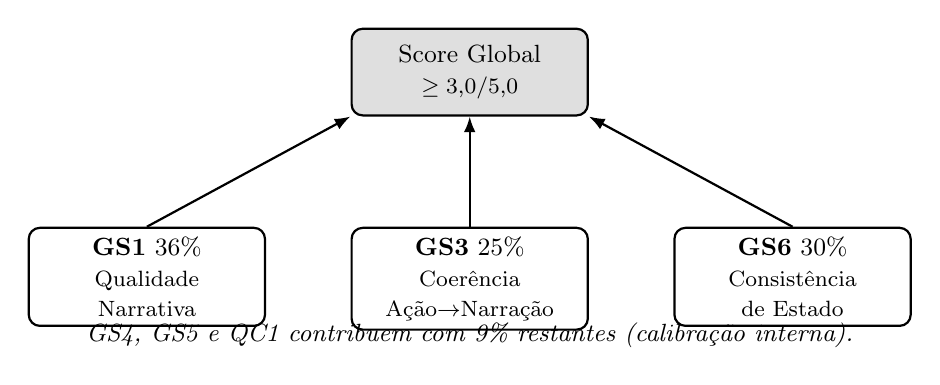
\begin{tikzpicture}[
  every node/.style={font=\small, align=center},
  box/.style={rectangle, rounded corners, draw=black, thick,
              minimum width=3.0cm, minimum height=1.1cm},
  top/.style={box, fill=gray!25},
  arr/.style={-{Latex[length=2mm]}, thick}
]
\node[top] (sg) {Score Global\\\footnotesize $\geq 3{,}0/5{,}0$};
\node[box, below=1.4cm of sg, xshift=-4.1cm] (gs1) {\textbf{GS1} 36\%\\\footnotesize Qualidade\\\footnotesize Narrativa};
\node[box, below=1.4cm of sg]                 (gs3) {\textbf{GS3} 25\%\\\footnotesize Coerência\\\footnotesize Ação$\to$Narração};
\node[box, below=1.4cm of sg, xshift=4.1cm]  (gs6) {\textbf{GS6} 30\%\\\footnotesize Consistência\\\footnotesize de Estado};
\draw[arr] (gs1.north) -- (sg.south west);
\draw[arr] (gs3.north) -- (sg.south);
\draw[arr] (gs6.north) -- (sg.south east);
\node[below=2.5cm of sg, font=\itshape\small] {GS4, GS5 e QC1 contribuem com 9\% restantes (calibração interna).};
\end{tikzpicture}
\caption{Estrutura ponderada das métricas do \texttt{rpg\_judge.py}. GS1+GS3+GS6 perfazem 91\% do score global, refletindo o foco em qualidade do GM LLM; as demais métricas medem calibração do sistema de avaliação interno.}
\label{fig:metricas}
\end{figure}

\subsection{LLM-as-a-Judge}

O modelo avaliador (\textit{judge}) recebe como entrada trechos da sessão---a ação do jogador e a narração gerada pelo MJ---acompanhados de instruções específicas para atribuição de notas em escala Likert (1--5). Cada prompt de avaliação é isolado por métrica, evitando que o contexto de uma avaliação influencie outra.

O mesmo backend LLM configurado em \texttt{llm\_config.py} pode ser utilizado tanto para geração quanto para avaliação. Embora isso introduza possível circularidade---o modelo tendendo a avaliar favoravelmente o que ele próprio geraria---essa abordagem é metodologicamente válida conforme Yu et al. \cite{yu:2025}, desde que documentada. Para mitigar o viés, recomenda-se usar modelos diferentes para geração e julgamento nas sessões de avaliação formal.

O \texttt{rpg\_judge.py} suporta filtragem por \texttt{session\_id} no \texttt{mundo\_log.csv}, garantindo que apenas eventos da sessão correspondente sejam avaliados nas métricas de mundo aberto (MW1, MW2).

\subsection{Mitigação de Alucinação}

Uma limitação observada em modelos \textit{reasoning} (Gemma~4, DeepSeek-R1, Qwen3) foi a tendência de inventar contexto narrativo não mencionado no prompt. A mitigação adotada---instrução explícita ``NUNCA invente personagens, eventos ou contexto não mencionados'' no \texttt{SYSTEM\_PROMPT\_NARRACAO}---reduziu os casos, mas não os eliminou completamente em modelos com temperatura $> 0{,}7$.

Modelos \textit{reasoning} também produzem blocos internos \texttt{<think>...</think>} antes de responder. O sistema filtra esses blocos via expressão regular após acumular todo o texto do \textit{stream}, evitando que tokens de raciocínio interno apareçam na narração exibida ao jogador.

% ─────────────────────────────────────────────────────────────────────────────
\section{Implementação}

O sistema foi implementado em Python, com o módulo \texttt{rpg\_judge.py} responsável pela avaliação automática. As sessões de jogo geram arquivos CSV estruturados com os seguintes campos: tipo de interação (\texttt{avaliacao}, \texttt{narracao\_jogador}, \texttt{narracao\_inimigo}, \texttt{questionario\_p1-5}, \texttt{mundo\_*}), entrada do jogador, resposta do MJ, tokens consumidos e tempo de resposta. A partir de Abril de 2026, os campos de entrada e resposta são registrados sem truncamento (até 2000 caracteres), garantindo que narrações completas estejam disponíveis para avaliação.

A arquitetura suporta três backends LLM: modelos locais via Ollama, servidores locais via LM Studio 0.4.11 e APIs externas (Groq). O sistema opera sem cache, lendo o backend e o modelo diretamente do \texttt{llm\_config.py} a cada chamada, permitindo troca dinâmica de modelos sem reinicialização.

\begin{footnotesize}
\begin{verbatim}
python rpg_judge.py logs/sessao_2026-04-18.csv
python rpg_judge.py logs/
# Saida: judge_results/rpg_judge_resultados.csv
#        judge_results/rpg_judge_agregado.json
\end{verbatim}
\end{footnotesize}

\section{Resultados}

A Tabela~\ref{tab:resultados} resume os resultados da avaliação preliminar. Os experimentos foram conduzidos sobre uma sessão de referência (69 entradas, 34 narrações, 5 perguntas do questionário) e sessões adicionais com modelos distintos, e apresentam os scores médios obtidos pelas três métricas dominantes e o score global agregado. Para interpretação da escala Likert (1--5): \textbf{scores próximos de 4 indicam desempenho narrativo consistente}, enquanto \textbf{valores abaixo de 3 revelam inconsistências frequentes} (contradições entre turnos, ações narradas incorretamente, ou narração genérica). O limiar de aprovação $\geq 3{,}0$ adotado em RPGBench \cite{yu:2025} marca o piso de utilidade do GM LLM.

\begin{table}[ht]
\centering
\caption{Resultados experimentais por modelo (escala Likert 1--5). $n$ = sessões avaliadas; \textbf{negrito} = melhor por coluna.}
\label{tab:resultados}
\small
\begin{tabular}{lccccc}
\toprule
\textbf{Modelo} & $n$ & \textbf{GS1} & \textbf{GS3} & \textbf{GS6} & \textbf{Global} \\
\midrule
\texttt{qwen2.5:7b-instruct}                           & 1 & \textbf{4{,}79} & \textbf{5{,}00} & 2{,}94          & \textbf{3{,}87} \\
\texttt{gemma4:e2b}~$^{\dagger}$ \cite{deepmind:gemma4:2026} & 1 & 4{,}54          & 4{,}84          & \textbf{2{,}97} & 3{,}70          \\
\texttt{qwen2.5:1.5b}                                  & 7 & 3{,}21          & 4{,}88          & 2{,}21          & 3{,}14          \\
\texttt{qwen2.5:0.5b}                                  & 1 & 3{,}34          & 3{,}52          & 2{,}04          & 3{,}07          \\
\bottomrule
\end{tabular}
\\[2pt]
{\footnotesize $^{\dagger}$ Avaliação obtida após adaptação do parser de saída do \texttt{rpg\_judge.py} para \textit{reasoning models} (\textit{strip} de blocos \texttt{<think>} e busca pelo último JSON balanceado), com taxa de sucesso de parse de 100\% (196/196 chamadas). Antes da adaptação, o mesmo modelo registrava Global $\approx 1{,}9$ devido a falhas de extração --- resultado de engenharia de integração, não de capacidade do modelo.}
\end{table}

\textbf{O \texttt{qwen2.5:7b-instruct} e o \texttt{gemma4:e2b} se destacam como os dois únicos modelos a ultrapassarem o limiar de aprovação ($\geq 3{,}0$) em todas as métricas dominantes, com perfis surpreendentemente próximos: 7B-instruct vence em GS1/GS3, e \texttt{gemma4:e2b} (effective 2B) vence em GS6 --- evidência direta de que arquitetura e regime de treino podem compensar diferença de parâmetros para consistência de estado.} O \texttt{qwen2.5:7b-instruct} fica em Global $=3{,}87$, com GS1 próximo do teto (4{,}79) e GS3 saturando em 5{,}00. O \texttt{gemma4:e2b} alcança Global $=3{,}70$ com a maior nota de GS6 da bateria (2{,}97). As variantes menores da família Qwen2.5 (1.5B e 0.5B) ficam pouco acima do limiar, com perfis distintos: \texttt{qwen2.5:1.5b} apresentou alta variância entre sessões (Global $\in [1{,}95;~3{,}72]$, $\sigma=0{,}81$, $n=7$), indicando sensibilidade ao histórico injetado e ao estilo do jogador. \textbf{Achado metodológico relevante:} o \texttt{gemma4:e2b} inicialmente registrou Global $\approx 1{,}9$ devido a um defeito de integração ---  o parser do judge não removia blocos \texttt{<think>...</think>} dos \textit{reasoning models} e capturava o primeiro \texttt{\{...\}} encontrado, frequentemente dentro do bloco de pensamento. Após a correção (\textit{strip} de \texttt{<think>} e busca pelo último JSON balanceado), o mesmo modelo saltou para 3{,}70 sem qualquer mudança no MJ ou no judge --- ilustrando que \textit{engenharia de integração} pode ser o limite efetivo, não a capacidade do modelo. \textbf{GS6 (consistência de estado) permanece como o gargalo principal:} mesmo o melhor modelo (\texttt{gemma4:e2b}) fica em $2{,}97$, no piso do limiar --- coerência de longo prazo continua sendo o limite duro de modelos de pesos abertos sub-10B. GS3 satura próximo de $5{,}00$ nos modelos $\geq 1{,}5$B, indicando que ações simples são fielmente narradas. Embora limitados em escala (quatro modelos, três cenários, $n=10$ sessões), estes resultados são suficientes para demonstrar a \textit{capacidade discriminativa} do protocolo proposto: as métricas separam modelos com perfis distintos de forma reprodutível e expõem o gargalo de consistência como direção prioritária para futuras versões.

\textbf{Modos de Falha Observados.} A análise qualitativa das sessões revelou cinco padrões sistemáticos de falha, mais frequentes em modelos abaixo de 7B: \textit{(i)} \textbf{vazamento de variáveis internas} --- o judge \texttt{qwen2.5:0.5b} adicionou ao JSON de saída um campo não solicitado (\texttt{"necessita de contexto envolvente"}), expondo critério interno de avaliação; \textit{(ii)} \textbf{persistência de alucinação via histórico contaminado} --- uma alucinação inicial (nome incorreto do jogador como \textit{``Silvano''}) propagou-se entre sessões e entre modelos distintos via histórico de mensagens, observada tanto em \texttt{qwen2.5:1.5b} quanto em \texttt{gemma4:e2b}; \textit{(iii)} \textbf{quebra de persona com meta-desculpas} --- \texttt{qwen2.5:1.5b} respondeu como assistente técnico (\textit{``Peço desculpas pela confusão anterior...''}) em vez de manter o NPC, expondo a razão de design da restrição (\textit{``poderia desencorajar visitantes''}); \textit{(iv)} \textbf{vazamento de prefixos do log} --- \texttt{gemma4:e2b} reproduziu literalmente os rótulos \texttt{Yara:} e \texttt{Fe:} do histórico estruturado, vazando a estrutura técnica do sistema; \textit{(v)} \textbf{admissão de limitação técnica} --- modelo justificou ausência de informação como \textit{``não tenho a capacidade''}, expondo o limite do prompt de sistema em vez de criar barreira narrativa. Quanto ao ritmo, falhas ocorreram \textbf{já no turno 0} quando o histórico de sistema injetado continha erros de testes anteriores, e \textbf{entre os turnos 1 e 4} em diálogos com NPCs por acúmulo de contexto excedendo a janela de atenção dos modelos pequenos para instruções negativas (\textit{``não saia da persona''}).

\textbf{Limitações.} É importante reforçar que \textit{LLM-as-a-judge não é \textit{ground truth}}: o judge fornece uma estimativa correlacionada --- não equivalente --- ao julgamento humano, e seus erros não são puramente aleatórios, mas sistemáticos. A abordagem apresenta quatro limitações principais: (1) \textit{viés do modelo avaliador} --- o judge tende a favorecer estilos próximos ao seu próprio padrão de geração; (2) \textit{dependência de prompts} --- pequenas variações no prompt de avaliação podem alterar significativamente as notas; (3) \textit{circularidade} --- quando o mesmo modelo base é usado para geração e julgamento, o sistema pode superestimar a qualidade das próprias narrações; (4) \textit{ausência de avaliação humana formal das narrativas} --- embora as sessões tenham sido conduzidas por 3 jogadores reais (introduzindo variância de estilo), \textbf{nenhuma escala subjetiva de imersão ou agência foi coletada dos jogadores}: o judge correlaciona com julgamento humano em tarefas abertas \cite{zheng:2023}, mas não substitui a percepção subjetiva. Validação cruzada com survey de jogadores é direção de trabalho futuro. O viés de circularidade é mitigado usando modelos diferentes para geração e julgamento nas sessões formais (\texttt{qwen2.5:7b-instruct} como judge, demais como geradores).

% ─────────────────────────────────────────────────────────────────────────────
\section{Conclusão}

Este trabalho apresentou um sistema de GM autônomo baseado em LLMs locais com três cenários de avaliação e o módulo \texttt{rpg\_judge.py} para avaliação automática via LLM-as-a-judge. A arquitetura de persistência em três camadas (SQLite, JSON, CSV) demonstrou-se eficaz para manutenção de consistência narrativa, e o sistema de avaliação implementa métricas comparáveis às propostas em RPGBench \cite{yu:2025}. \textbf{O protocolo proposto não se restringe a RPGs}: a estrutura de logs estruturados, métricas ponderadas e LLM-as-a-judge é aplicável a outros sistemas interativos baseados em LLM (assistentes narrativos, agentes conversacionais de longa duração, simulações de role-play educacional), ampliando seu potencial de impacto além do escopo deste trabalho.

Como trabalho futuro, pretende-se: (1) validação com avaliadores humanos para correlacionar as métricas automáticas com percepção subjetiva de qualidade; (2) uso de múltiplos modelos \textit{judge} para reduzir o viés de circularidade e aumentar a robustez das avaliações; (3) refinamento das métricas narrativas com análise de diversidade lexical (TTR, MTLD) conforme Reviriego et al. \cite{reviriego:2024}; (4) integração de banco vetorial FAISS para memória semântica de longo prazo; (5) expansão do Cenário C com encontros de diálogo no mundo aberto.

\textbf{Agradecimentos.} [OMITIDO PARA REVISÃO ANÔNIMA]

\bibliographystyle{sbc}
\bibliography{Referencias/referencias}

\end{document}
